\chapter{Physical Form}
% TODO: Add scale to photos
To enable the prototype to be easily mounted on the ceiling, the prototype was placed on a flat board with feet that would enable it to be screwed into a pole, and the pole extended to jam the sensor against the ceiling and the floor using the pole (\Fref{fig:pictures:protob1}, \Fref{fig:pictures:protoact}). Due to a wireless module and battery pack being added to the Raspberry Pi, it was feasible for the sensor to operate entirely wirelessly for several hours. However, in most cases it was more convenient to operate using wired power and Ethernet.

\begin{figure}[H]
\centering
\includegraphics[height=0.5\textheight]{../diagrams/prototype-mounted-ceiling.jpg}
\caption{Prototype in action}
\label{fig:pictures:protoact}
\end{figure}

\begin{figure}[H]
\centering
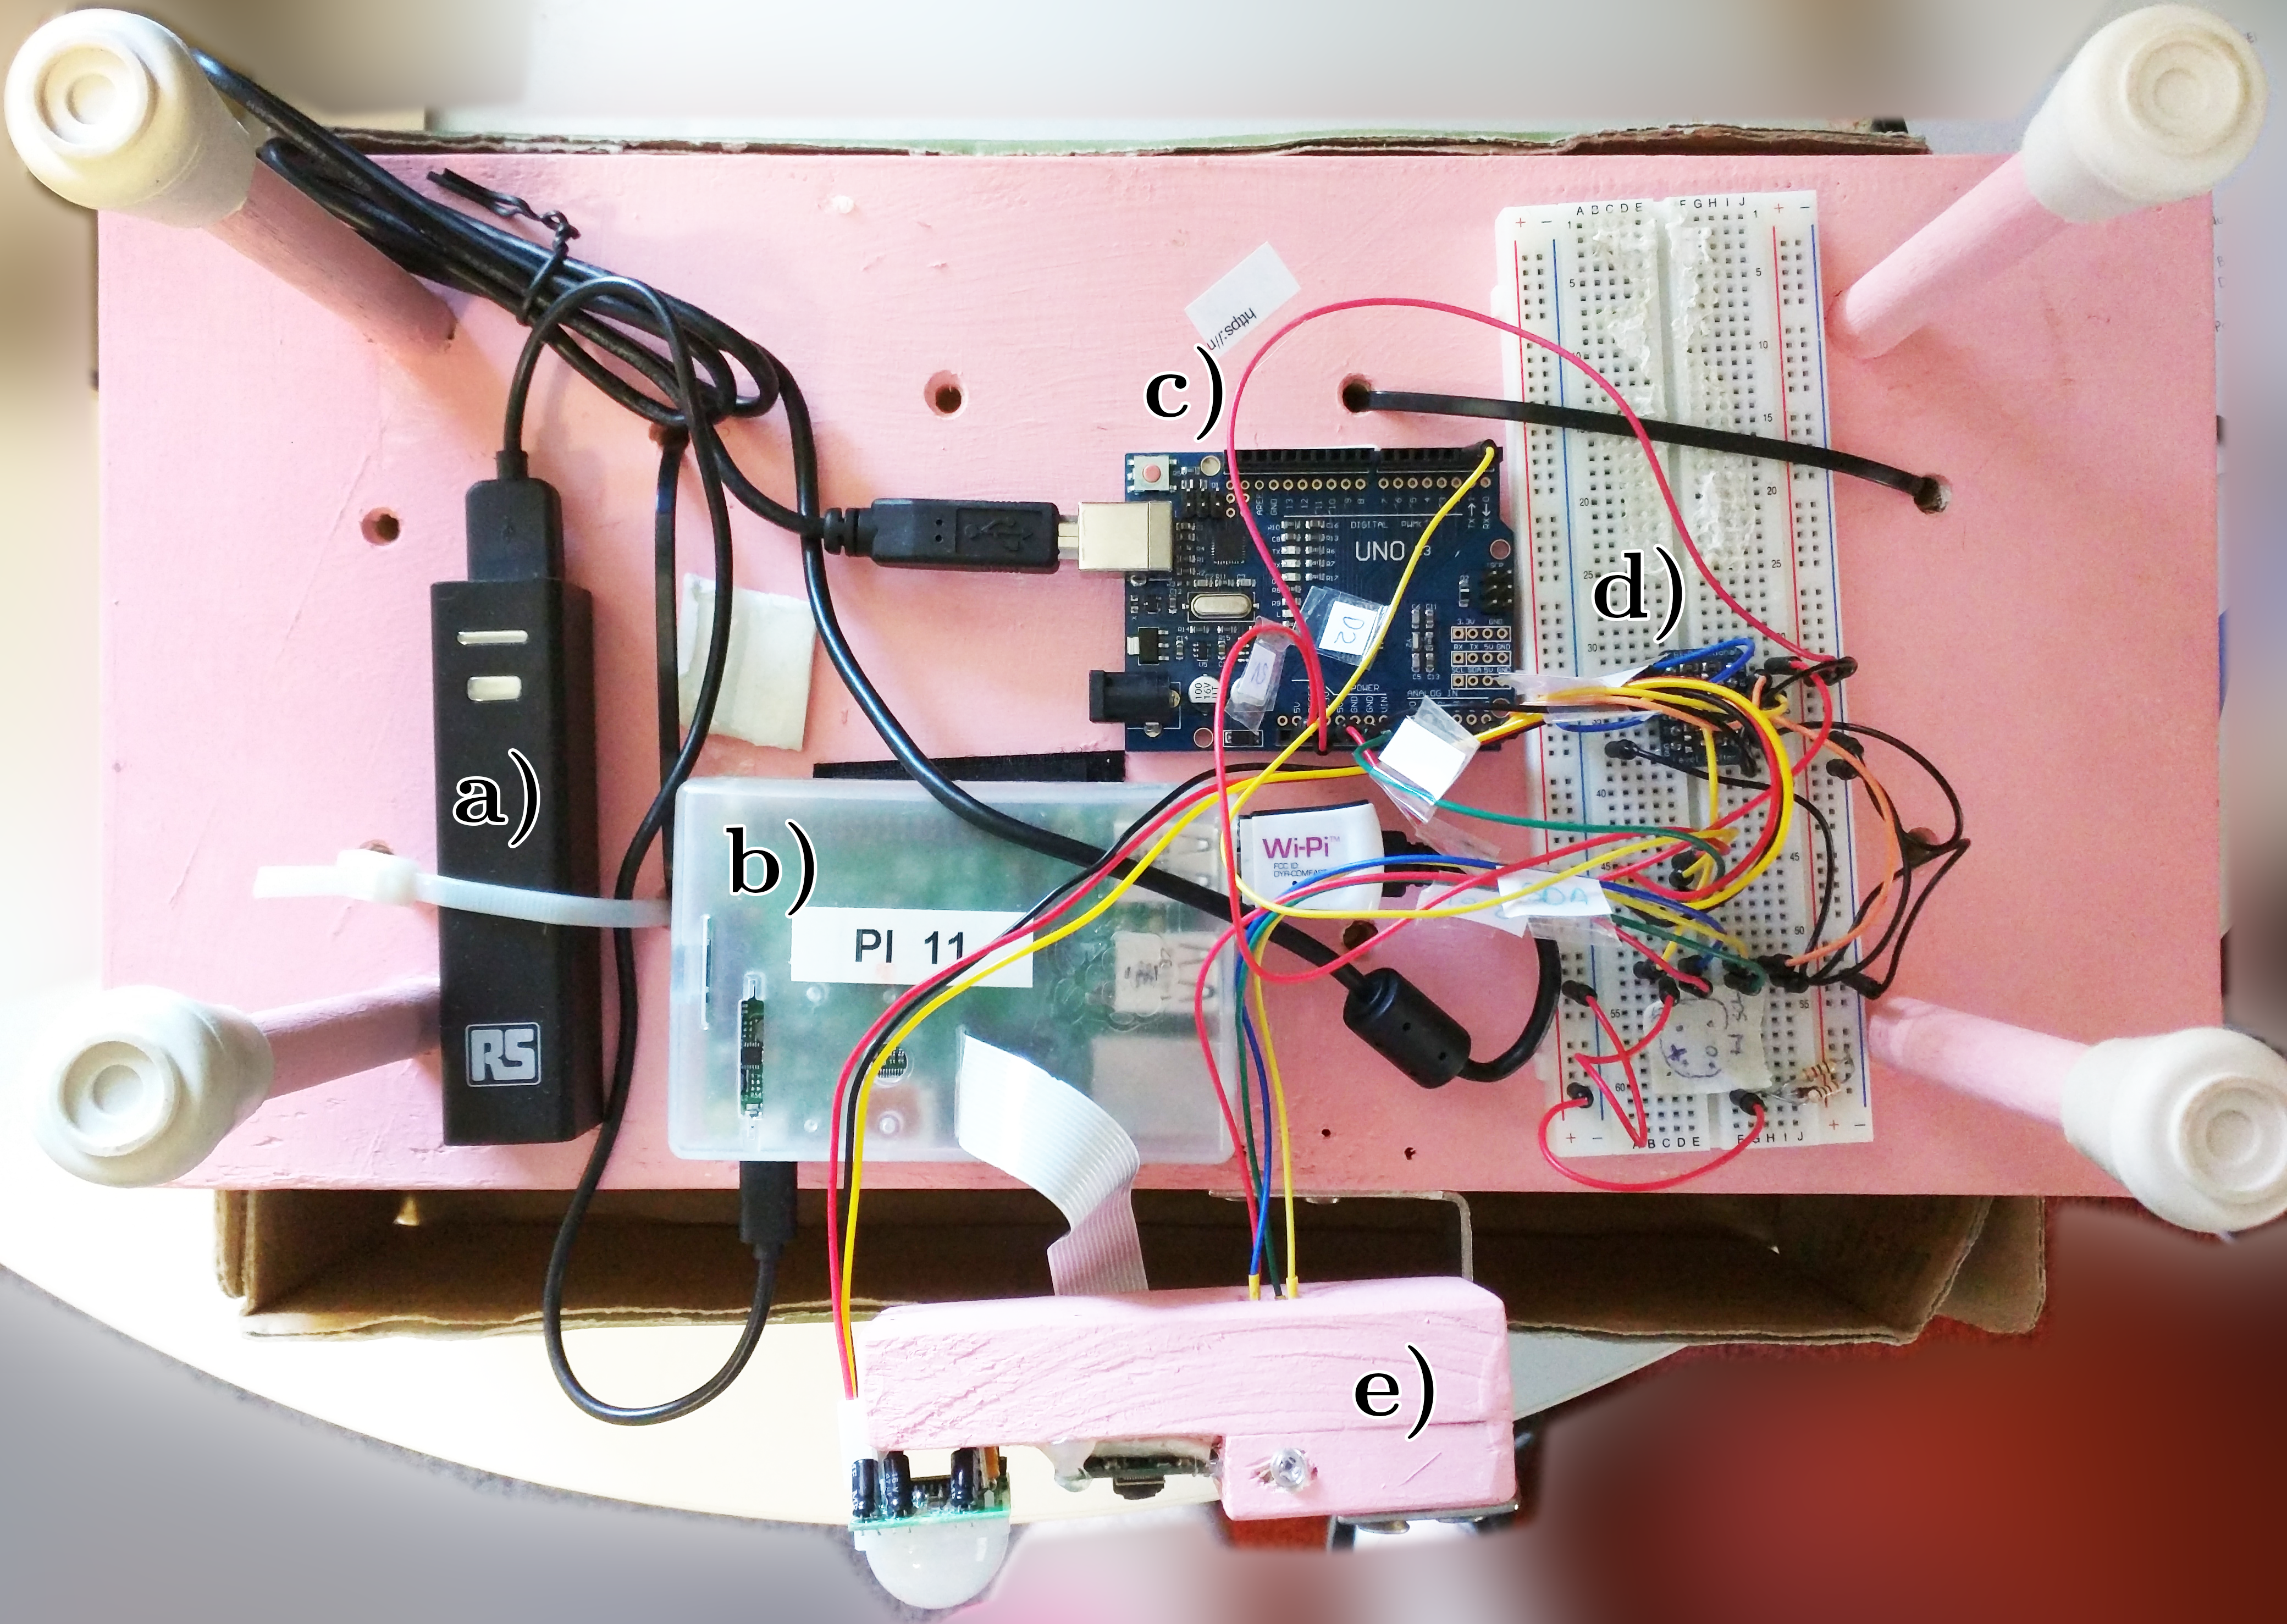
\includegraphics[width=\textwidth]{../diagrams/prototypeb-1.jpg}
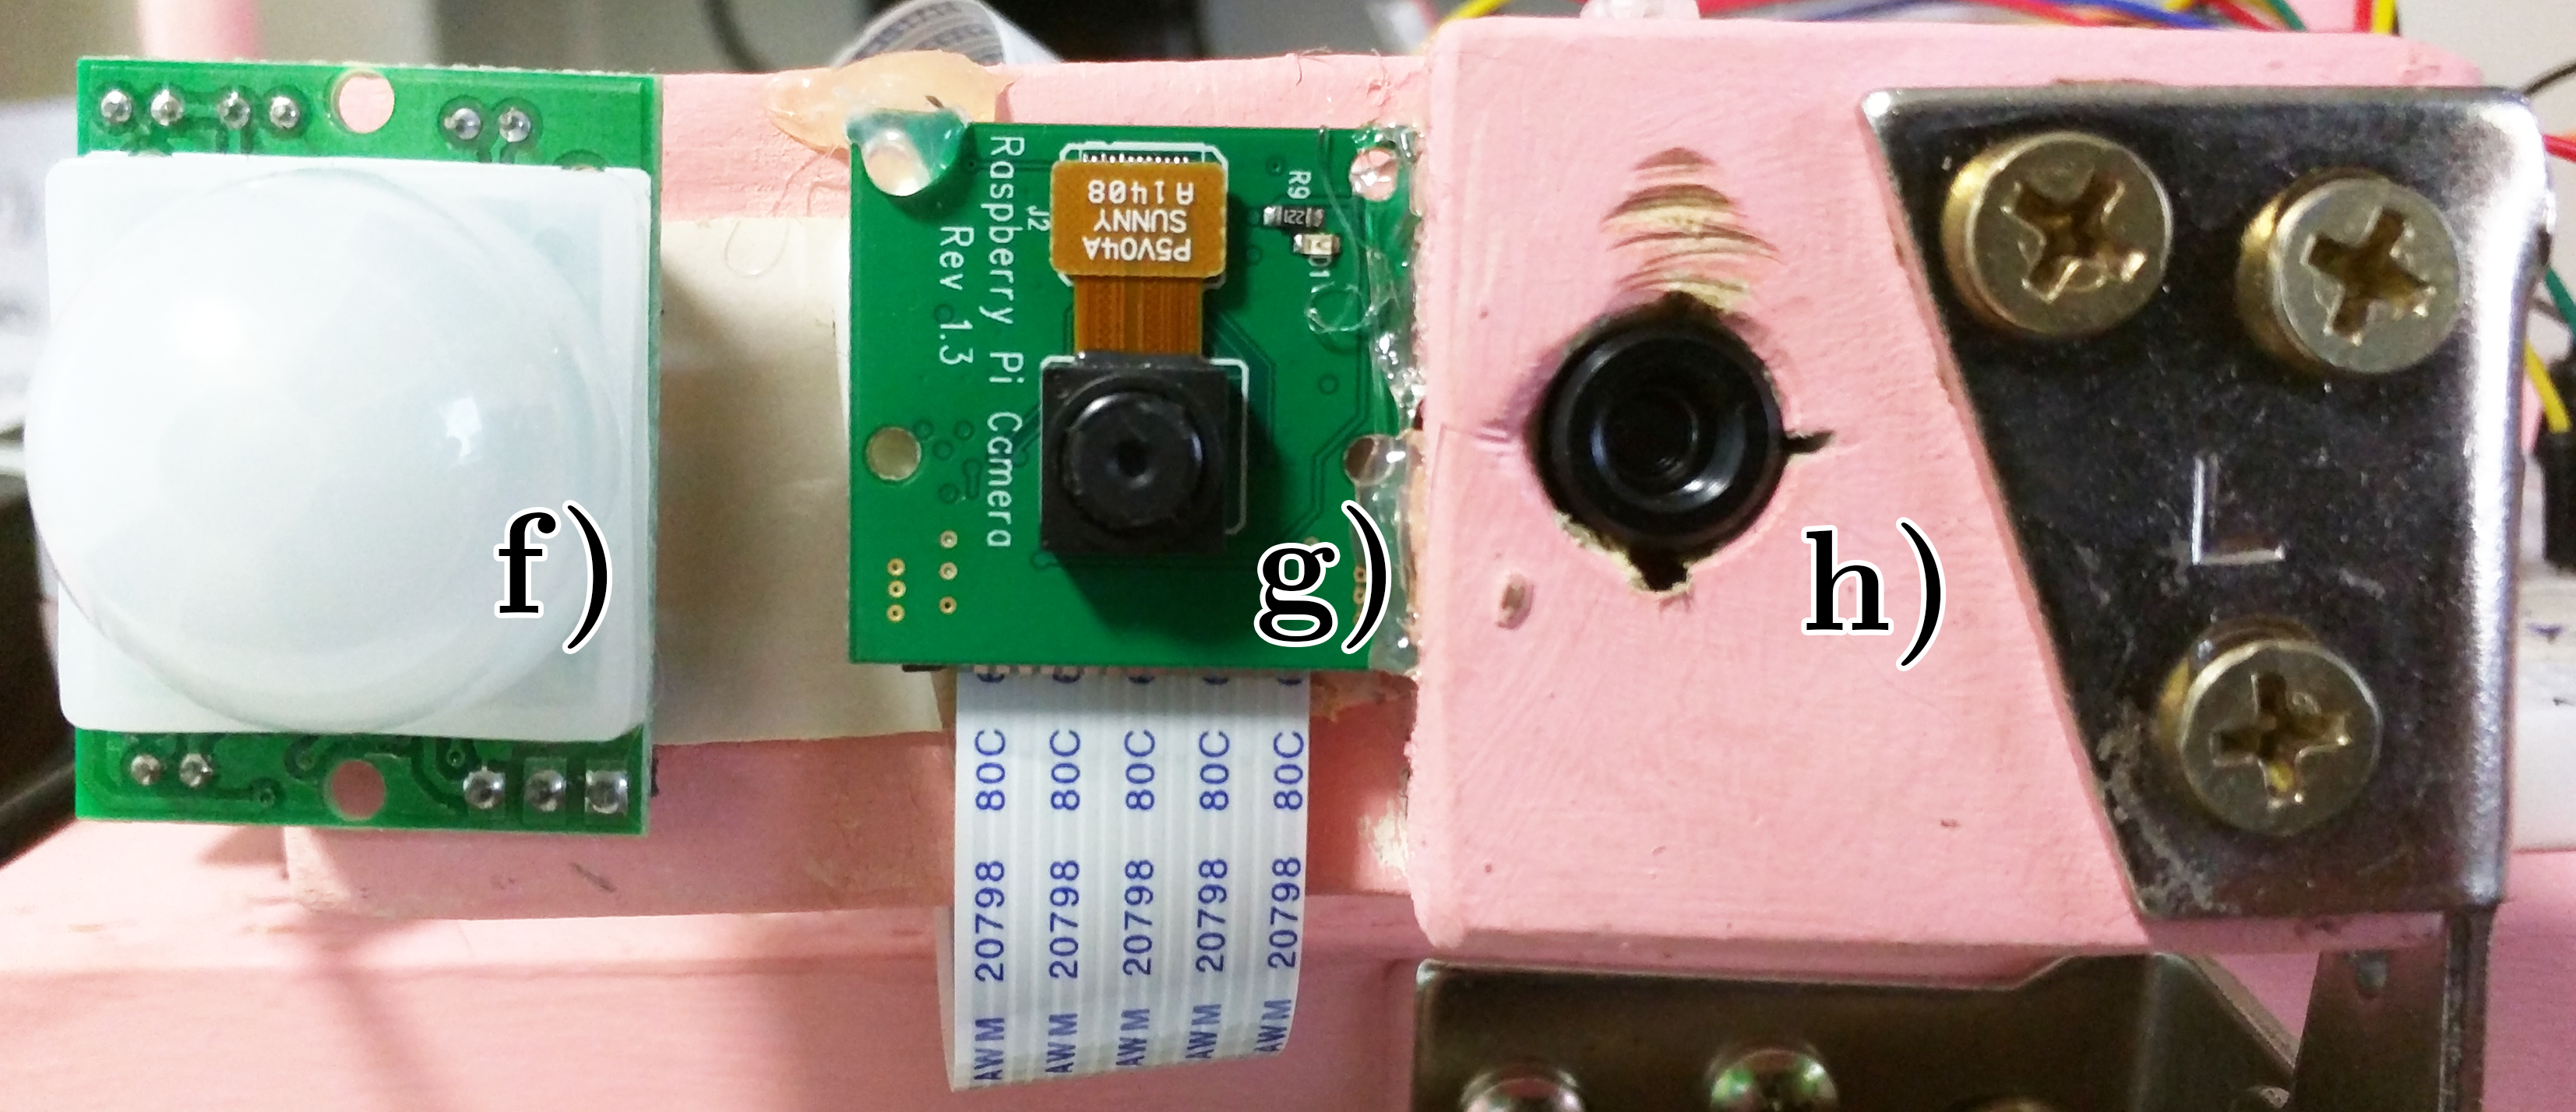
\includegraphics[width=\textwidth]{../diagrams/prototypeb-2.jpg}
{\small
\begin{multicols}{2}
\begin{enumerate}[a)]
 \item Battery pack
 \item Raspberry Pi
 \item Arduino
 \item Level-shifting circuitry
 \item Movable sensor mount
 \item PIR
 \item Camera
 \item \mlx
\end{enumerate}
\end{multicols}
}
\caption{Prototype Physical Form}
\label{fig:pictures:protob1}
\end{figure}

\begin{landscape}
\chapter{Knowledge Flows}
\label{chap:knowledgeflows}

\begin{figure}[H]
\centering
\includegraphics[width=\linewidth]{../diagrams/knowledgeflow-numeric.png}
\caption{Numeric knowledge flow}
\end{figure}
\end{landscape}

\begin{landscape}
\begin{figure}[H]
\centering
\includegraphics[width=\linewidth]{../diagrams/knowledgeflow-nominal.png}
\caption{Nominal knowledge flow}
\end{figure}

In Weka, Knowledge Flows can be defined, which provide an easy way to replicate a series of Weka functions. We provide a unified knowledge flow at the \texttt{run\_flow.py} script to execute it on a given data set. However, we also replicate the numeric and nominal flows here (separated due to size) for those interested.
\end{landscape}

\chapter{Original Honours Proposal}
\subfile{../proposal/proposal}